\chapter{Einleitung}
Durch den stetigen Fortschritt und der steigenden Komplexität der Anwendungen
werden große Datenmengen erzeugt. Sei es im privaten Umfeld durch die Benutzung
von Social-Media Platformen wie Facebook, Twitter,~\dots oder im gewerblichen
Umfeld durch medinische Daten, Börsendaten,~\dots . Durch die stetige Vernetzung
von Alltagsgegenständen, welches man unter dem Begriff IoT\footnote{Internet of the Things}
zusammenfassen kann, steigen diese Datenmengen nochmals sehr stark an. Dies hat
zur Folge, dass die Verarbeitung dieser Datenmengen immer komplexer wird und dies
mit nur einem einzelnen Rechner nicht mehr möglich ist. Dies wird als BigData
bezeichnet. Bei der Verarbeitung von großen Datenmengen wird unterschieden
zwischen Batch-Processing und Stream-Processing. Beim Batch-Processing wird eine
feste Datenmenge in kleinere Einheiten unterteilt. Diese Teildaten werden dann
von mehreren Rechnern einzeln bearbeitet und anschließen die Ergebnisse wieder
kombiniert. Beim Stream-Processing gibt es keine feste Menge, sondern die Daten
kommen kontinuierlich in die Verarbeitung. Dadurch ist eine Echtzeitverarbeitung
möglich.

\begin{figure}
\centering
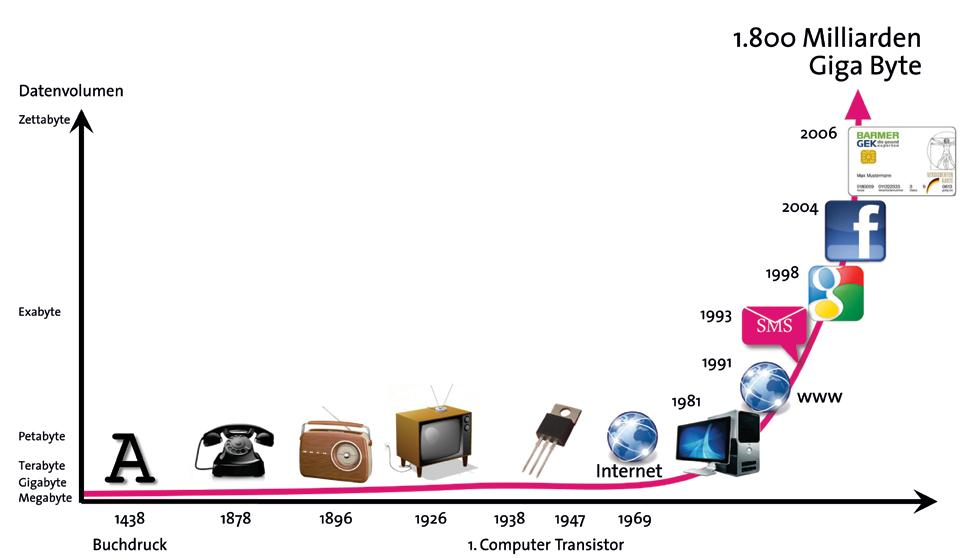
\includegraphics[scale=0.375]{images/bitkom-lf-bigdata-2012-data_grow.jpg}
\caption{Erhöhung der Datenmenge von 1400 bis 2006 \parencite{Weber2012}}
\label{fig:data-grow}
\end{figure}

Die Daten haben dabei je nach Anwendungsfall unterschiedlich strukturiert sein.
Es wird dabei unterscherschieden zwischen unstrukturierten, semi-strukturieren
und strukturierten Daten. Strukturierte Daten haben eine feste Struktur. Bei
semi-strukturieren Daten sind lediglich einzelen Bausteine definiert,
jedoch nicht wie die Daten aus den Bausteinen entstehen. Bei unstrukturierten
Daten ist lediglich die Information vorhanden, um welche Art von Daten es sich
handelt.

In der heutigen Welt spielen vor allem Graphen eine entscheidene Rolle. Da 
Unternehmen heute die Daten aus verschiedenen Quellen kombinieren wollen, um zum
Beispiel zusätzliche Werbung zu schalten. Als Beispiel jemand kauft ein Paar
Schuhe und bekommt dazu ein Angebot zu einer Tasche angezeigt, weil zum
Beispiel anderen Kunden beide Artikel gekauft haben. Ein anderes Beispiel von
Facebook ist die Liste der Personen, welche der Benutzer eventuell kennt.
Dabei werden die Informationen des Benutzers mit den Informationen der Freunde
bzw. deren Freunde kombiniert. Existiert nun eine Person, welche zum Beispiel
in die selbe Schule gegangen ist und nur Freund eines Freundes ist, wird diese
Person der Liste der Personen hinzugefügt, welche der Benutzer eventuell kennt.

Was sind nun eigentliche Graphen? Ein Graph ist eine Datenstruktur, welche aus
einer Menge von Knoten und einer Menge von Kanten besteht. Knoten sind die
Datencontainer. Zwei Knoten können dabei durch eine oder mehrere Kanten miteinander
verbunden sein. Jede Kante kann dabei gerichtet oder ungerichtet sein und
optionale Informationen enthalten sogenannte Gewichte. Diese spielen zum Beispiel
in der Routenplannung eine Rolle. Dort sind die Gewichte, die Entfernung in
Kilometern zwischen zwei Orten bzw. der Treibstoffverbrauch. Je nach dem welche
Arten von Kanten zulässig sind, werden die Graphen definiert. Bei einfachen
Graphen sind Schleifen und mehrfache Kanten verboten im Gegensatz zu komplexeren
Graphen.

\section{Motivation}
Wenn beide Welten BigData und Graphen mit einander kombiniert werden, ergeben
sich die verschiedene Problem. Zwei Probleme, die eng miteinander in Verbindung
stehen sind die Darstellung von Graphen und die Algorithmen.

%% Data-Warehouse, Tabelle -> Stream

\section{Ziel der Arbeit}

\section{Aufbau der Arbeit}
Im nächsten Kapitel werden die verwendeten Technologien und Softwaresysteme
beschrieben um einen Überblick zu bekommen. Dann wird dass Design der einzelnen
Beispiele erläutert und die sich schon abzeichnenden Probleme werden beschrieben.
Danach wird das Design anhand der technischen Umsetzung dargelegt, dabei werden
die auftretenden Probleme beschrieben. Abschliend folgt eine Zusammenfassung und
ein Ausblick auf zukünfgtige Schritte.
